\chapter{Results and Discussion} % Main chapter title

\label{Chapter5} % Change X to a consecutive number; for referencing this chapter elsewhere, use \ref{ChapterX}

\section{Solvation free energies}

The first part of this work consisted of obtaining phenanthrene parameters for the SAFT-$\gamma$ Mie Force Field, as  described in section \ref{parame}, since the parameters were not available for the ring geometry on the force field database. The parameters obtained and the mean percentage error (MPE) to the experimental data were:

\begin{table*}[h]
	\centering
	\caption{Estimated SAFT-$\gamma$ Mie Force Field parameters for phenanthrene}
	\label{tbl:estimparameters}
	\begin{tabular}{lllll}
		\hline
		 $m_s$ & $\epsilon/k_{B}$ (K) & $\sigma (\dot{A})$ & $\lambda_r$& MPE(\%) \\ \hline
		 3 \cite{lafitte2012}    & 485.55              & 4.197              & 14.34 & 1.64|9.74       \\ 
		 5  \cite{muller2017}   & 262.74               & 4.077              & 9.55   &  0.88   \\ \hline
	\end{tabular}
	
\end{table*} 

In the table above, the first value of MPE for the \citeonline{lafitte2012} strategy corresponds to the estimation with experimental data and the second corresponds to the corrections factors estimation with MD data. This strategy has an inconsistency of requiring two estimations because parameters solely  estimated with the EoS aren't accurate for molecular simulation. Hence, the solvation free energy of phenanthrene was only studied with the set of parameters estimated with \citeonline{muller2017} strategy. In fact, the \cite{lafitte2012} strategy was only followed because it was the only one available when we first started this work. The sets of parameters for the other compounds were retrieved from the literature \cite{lobanova2016,herdes2015,ervik2016,muller2017}:

\begin{table*}[h]
\centering
  \caption{SAFT-$\gamma$ Mie Force Field for each substance used in this work}
  \label{tbl:parameters}
  \begin{tabular}{lllll}
  	\hline
  	               & $m_s$ & $\epsilon/k_{B}$ (K) & $\sigma (\dot{A})$ & $\lambda_r$ \\ \hline
  	Water          & 1     & 305.21               & 2.902              & 8.0         \\
  	Propane        & 1     & 426.08               & 4.871              & 34.29       \\
  	Carbon dioxide & 2     & 194.94               & 2.848              & 14.65       \\
  	Hexane         & 2     & 376.35               & 4.508              & 19.57       \\
  	Octanol        & 3     & 495.71               & 4.341              & 28.79       \\
  	Toluene        & 3     & 268.24               & 3.685              & 11.80       \\
  	Benzene        & 3     & 230.30               & 3.441              & 10.45       \\
  	Pyrene         & 4     & 459.04               & 4.134              & 15.79       \\
  	Anthracene     & 5     & 259.68               & 3.631              & 9.55        \\ \hline
  \end{tabular}

\end{table*}

The solvation free energies of aromatic solutes in nonpolar (hexane), aromatic (toluene) and hydrogen bonding (1-octanol) solvents were examined with binary interaction parameters equal to zero. Since the force field doesn't account for charges, the solvation free energy is equal to the Mie contribution ( Eq. \eqref{eq:softcore}). A total of 15-18, depending on the pairs solute-solvent,  $\lambda s$ and their respective $\eta s$ were estimated as described in the methodology. The final $\lambda$ set was found using  
the cumulative probability distribution (Eq. \eqref{eqn:cumfun}) for all the pair. The distribution for the pair hexane+benzene can be seem in \figref{fig:optimized_cdf}. The final values of $\lambda$ and were concentrated on the region with a steeper slope as can been seen for the same pair solvent + solute in the Table \ref{tbl:lambdahex}.

\begin{figure}[h]
\centering
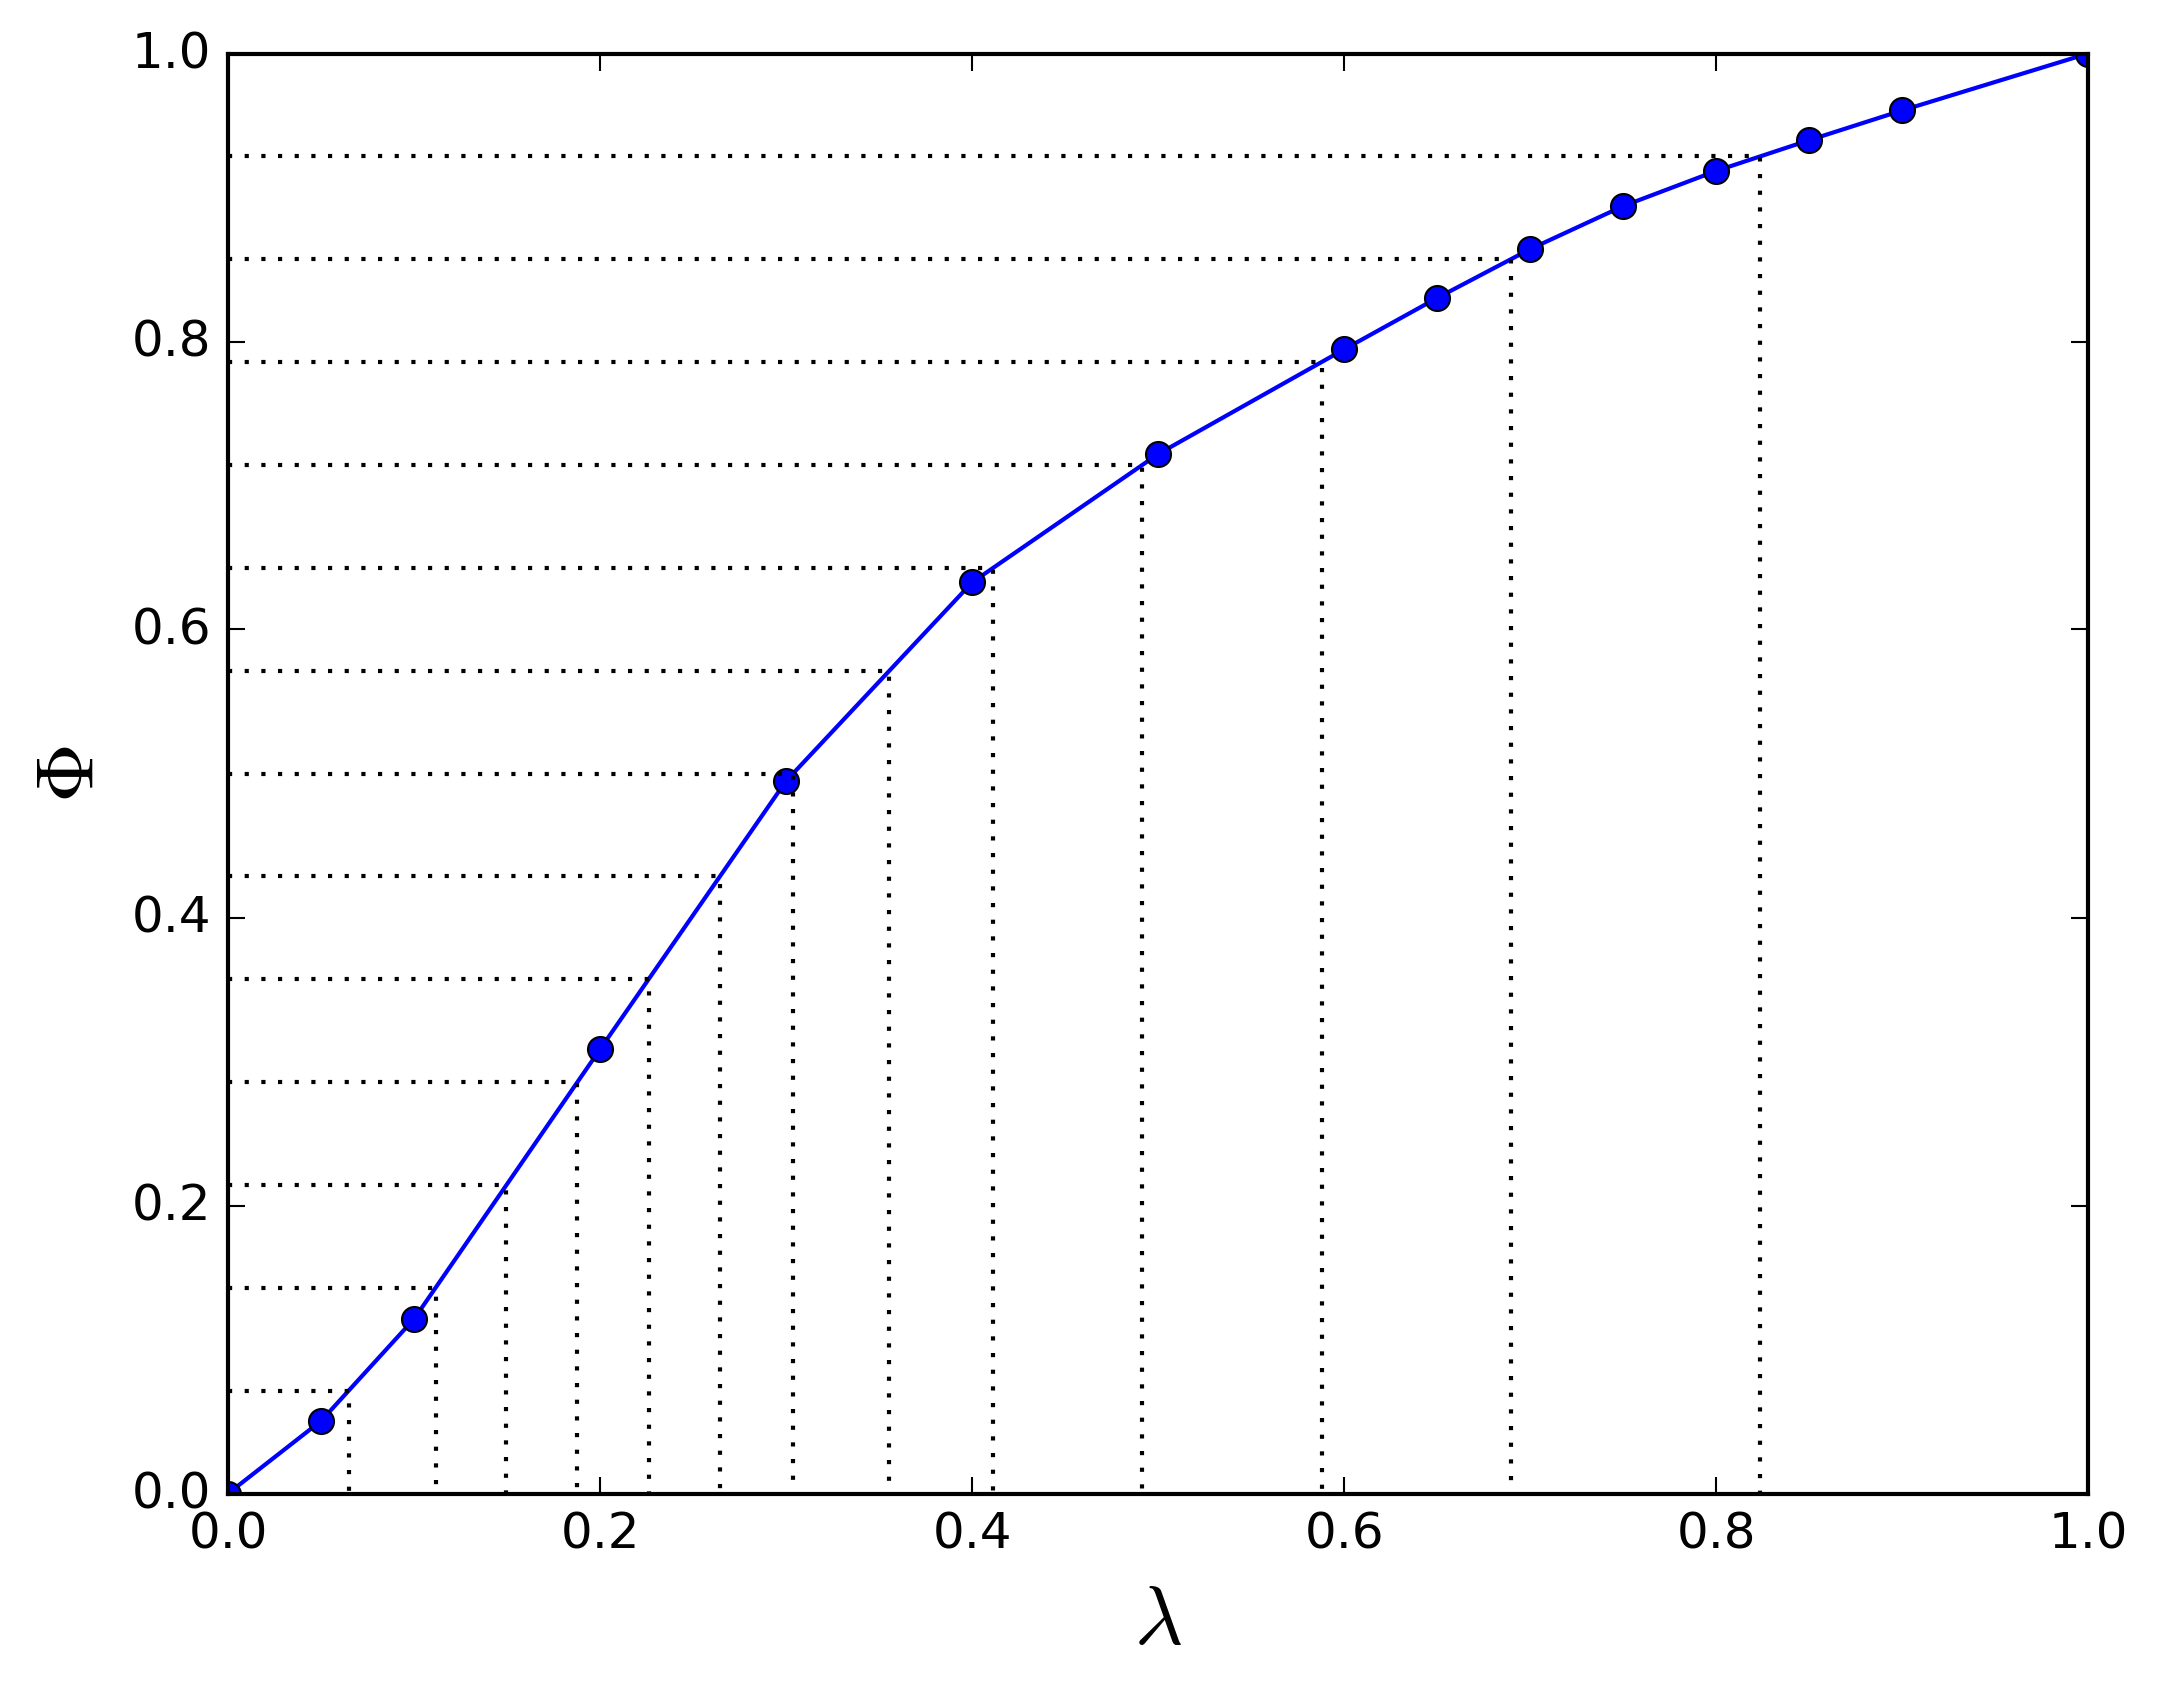
\includegraphics[width=0.7\linewidth]{Figures/optimized_cdf}
\caption{Cumulative probability}
\label{fig:optimized_cdf}
\end{figure}

\begin{table*}[h]
	\centering
	\caption{Optimized values of $\lambda$ and $\eta$ for the pair benzene + hexane}
	  \label{tbl:lambdahex}
	\begin{tabular}{ll}
		\hline
        $\lambda$	&	$\eta$\\ 
        \hline		
        0	&	0\\ 
        0.065	&	0.708\\ 
        0.112	&	1.385\\ 
        0.15	&	1.892 \\ 
        0.188	&	2.399\\ 
        0.226	&	2.519\\ 
        0.264	&	2.457\\ 
        0.304	&	2.367\\ 
        0.356	&	1.921\\ 
        0.411	&	1.411\\ 
        0.492	&	0.524\\ 
        0.588	&	-0.663\\ 
        0.69	&	-2.016 \\ 
        0.824	&	-3.922\\ 
        1	    &	-6.583\\ 	
		\hline
	\end{tabular}
\end{table*}

The $\lambda s$ and $\eta s$  for the other pairs are available at  Appendix A. It is also important to analyze the reliability of solvation free energy estimations  through the overlapping of the intermediate states. Insufficient overlap among states when using a FEP based such MBAR may result in the underestimation of variance, and, consequently, in the substantially incorrect free energies. The overlapping matrix for the solvation free energy of benzene in hexane is presented in Figure \figref{fig:hexove} and the matrices for the other pairs are available at Appendix B. The elements of these matrices are the probabilities of observing a sample from state  i in state j. As an example, the probability of observing state 6 in a simulation of state 8 is 0.16 in Figure \figref{fig:hexove}. It can be observed in the figures that  the matrices for all the pairs in this work have more than  three diagonals. In addition to that,  the probabilities in the three main diagonals are higher than 0.03, which indicates that the free energy estimations are reliable \cite{klimovich}.   

\begin{figure}[H]
	\centering
	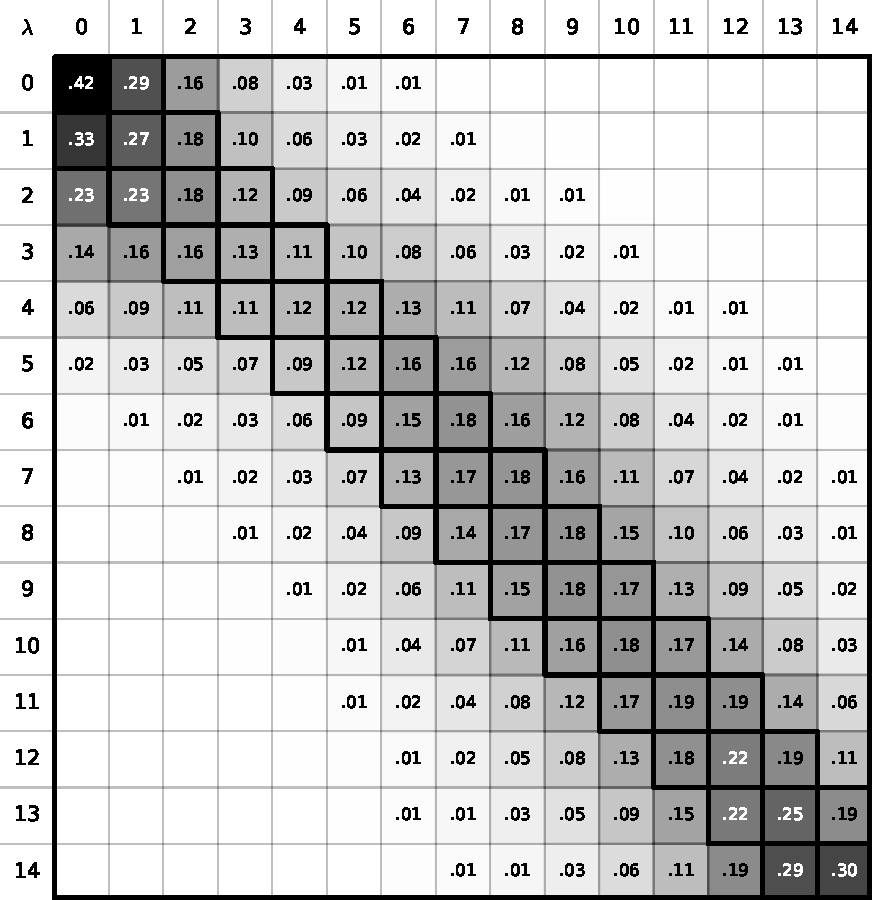
\includegraphics[width=0.8\textwidth]{Figures/ohex_benz}
	\caption{Overlapping matrix for hexane+benzene.}
    \label{fig:hexove}
\end{figure}

\begin{table*}[h]
\centering
  \caption{Calculated and experimental values for the solvation free energy differences (kcal/mol) of solutes in non aqueous solvents}
  \label{tbl:solv1}
  \begin{tabular}{lllll}
    \hline
      Solvent & Solute & $\Delta G_{solv}^{exp}$ & $\Delta G_{solv}^{Mie}$ & Absolute \\
      & & & & Deviation \\
    \hline
    hexane    & benzene      & -3.96  & -3.76  $\pm$ 0.01 & 0.20 \\
    hexane    & pyrene       & -11.53 & -10.82 $\pm$ 0.02 & 0.71 \\
    hexane    & phenanthrene & -10.01 & -9.16  $\pm$ 0.01 & 0.85 \\
    1-octanol & propane      & -1.32  & -1.36  $\pm$ 0.02 & 0.04 \\
    1-octanol & anthracene   & -11.72 & -8.16  $\pm$ 0.03 & 3.61 \\
    1-octanol & phenanthrene & -10.22 & -8.34  $\pm$ 0.03 & 1.47 \\
    toluene   & pyrene       & -12.86 & -11.74 $\pm$ 0.01 & 1.11\\
    toluene   & anthracene   & -11.31 & -9.90 $\pm$ 0.01 & 1.41\\
%    \hline
%    RMSE      &              &        &                   & 1.48     \\
    \hline
  \end{tabular}
\end{table*}

The numerical values for solvation free energies estimated in Table \ref{tbl:solv1} had smaller absolute deviations to experimental data, what shows that the SAFT-$\gamma$ Mie force field performs better for a non polar solvent. Additionally, this force field presented better results for the pair hexane+benzene than the Trappe force field \cite{garrido2011}. We also observed the effect of molecule's size on the entropic region of the free energy curve in Figure \ref{fig:hex}. It was expected that a force field based on an EoS that doesn't explicitly account for hydrogen bond would not perform well for 1-octanol. Despite this, the solvation free energies of propane and phenanthrene in 1-octanol stayed in the desired deviation range of 1-2 kcal/mol \cite{doimobley}. The deviation was much smaller for propane. This can be attributed to propane's non polarity and smoother free energy curve (Figure \ref{fig:oct}). The anthracene and phenanthrene molecules have the same geometry in the model and similar physical properties, but the absolute deviation of the solvation free energy of anthracene in 1-octanol is much higher than the one of phenanthrene 1-octanol. This may indicate a problem in the parameterization of anthracene.     

\begin{figure}[H]
\centering
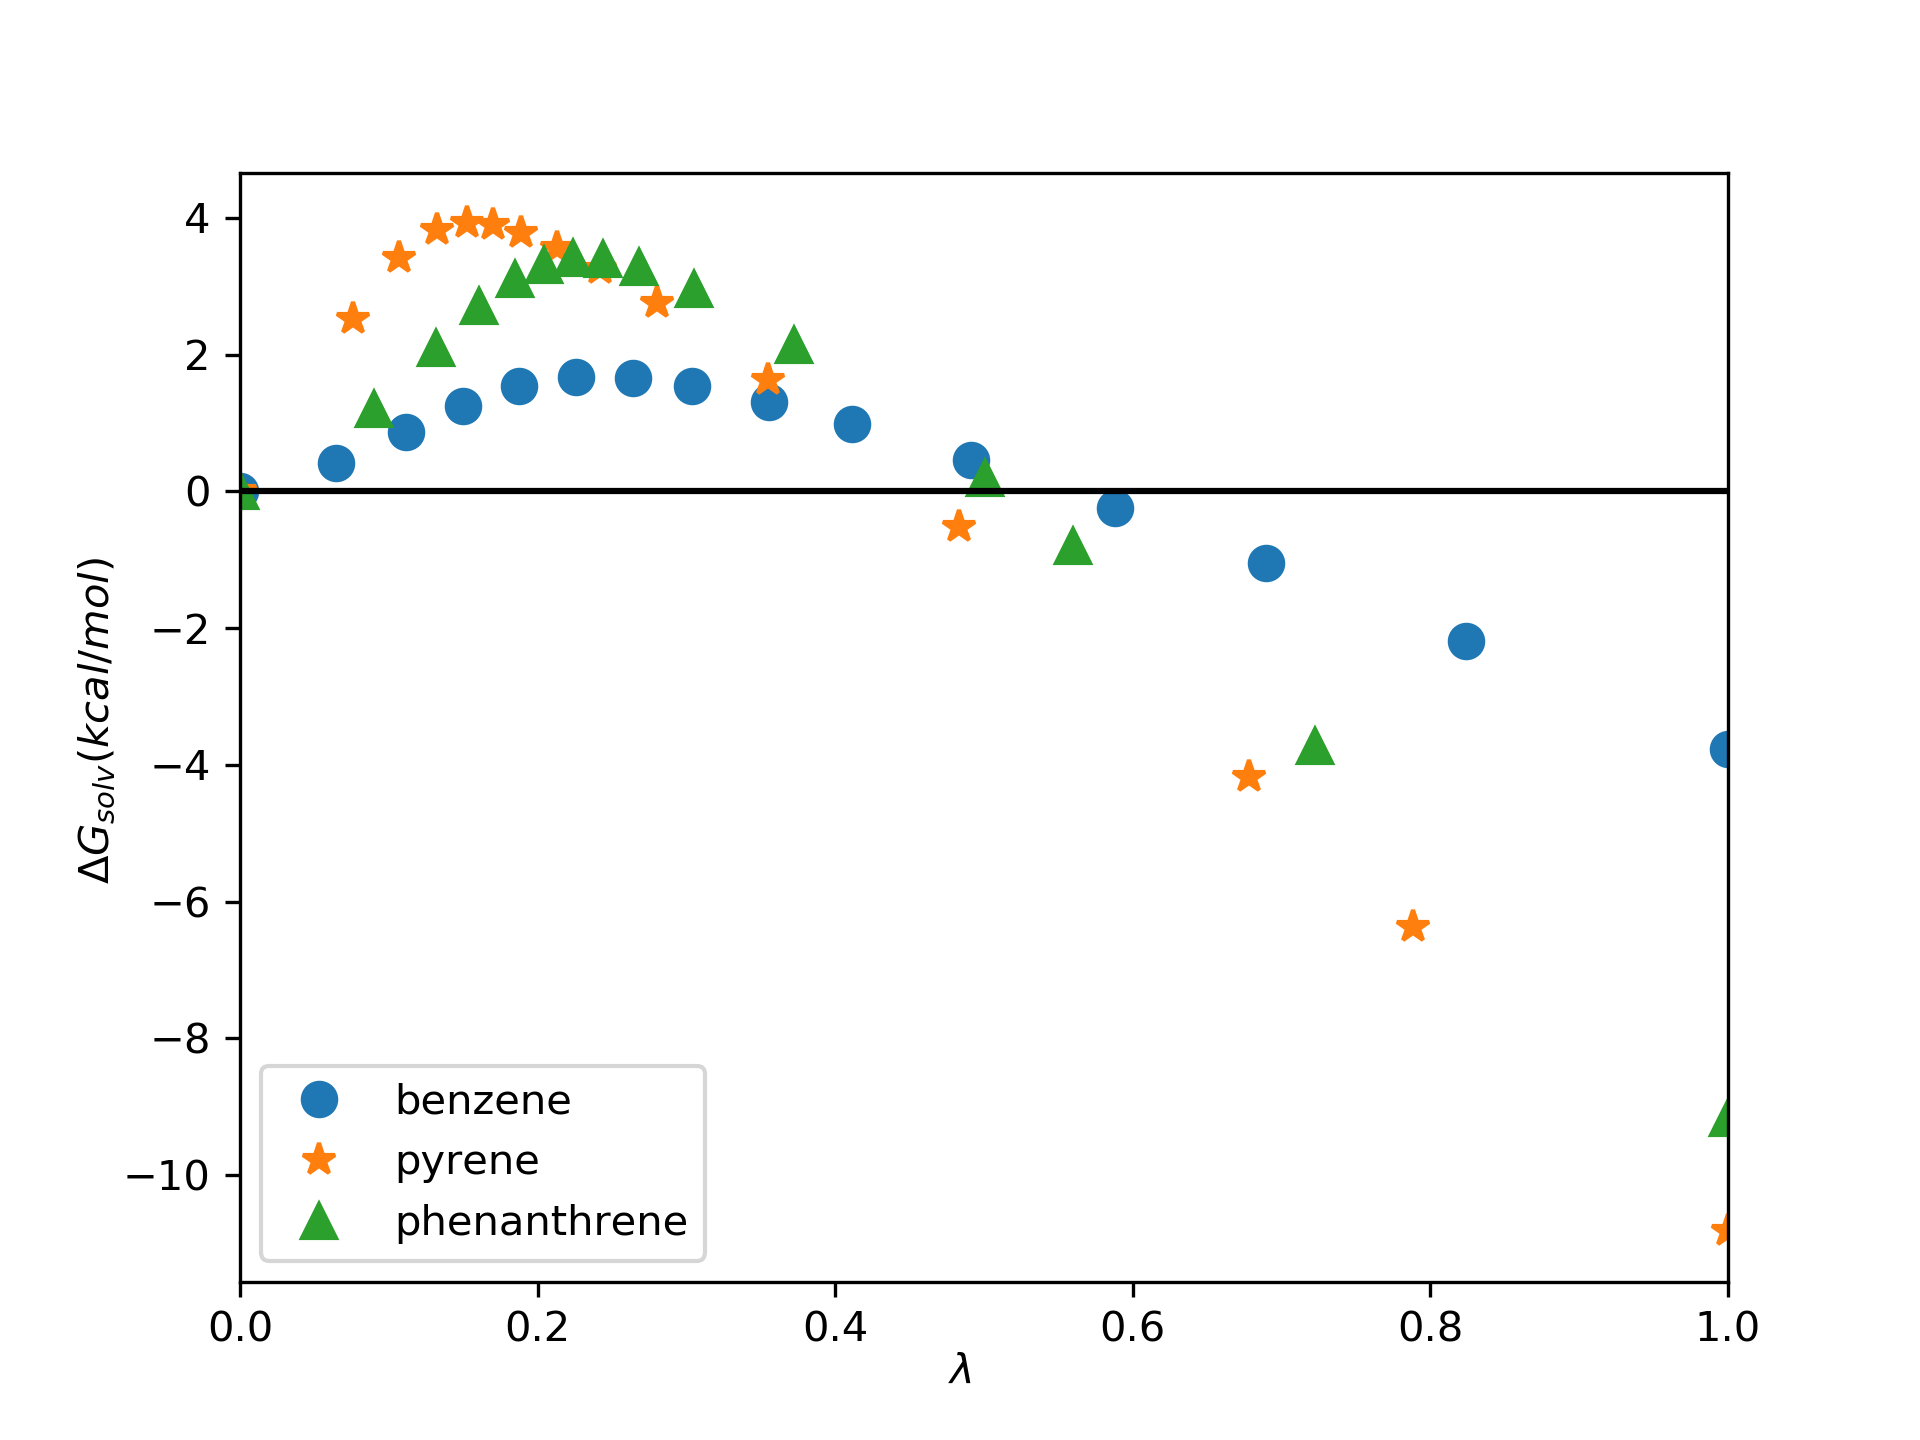
\includegraphics[width=0.9\linewidth]{Figures/hex}
\caption{Solvation free energy profiles of different solutes in hexane.}
\label{fig:hex}
\end{figure}

\begin{figure}[H]
	\centering
	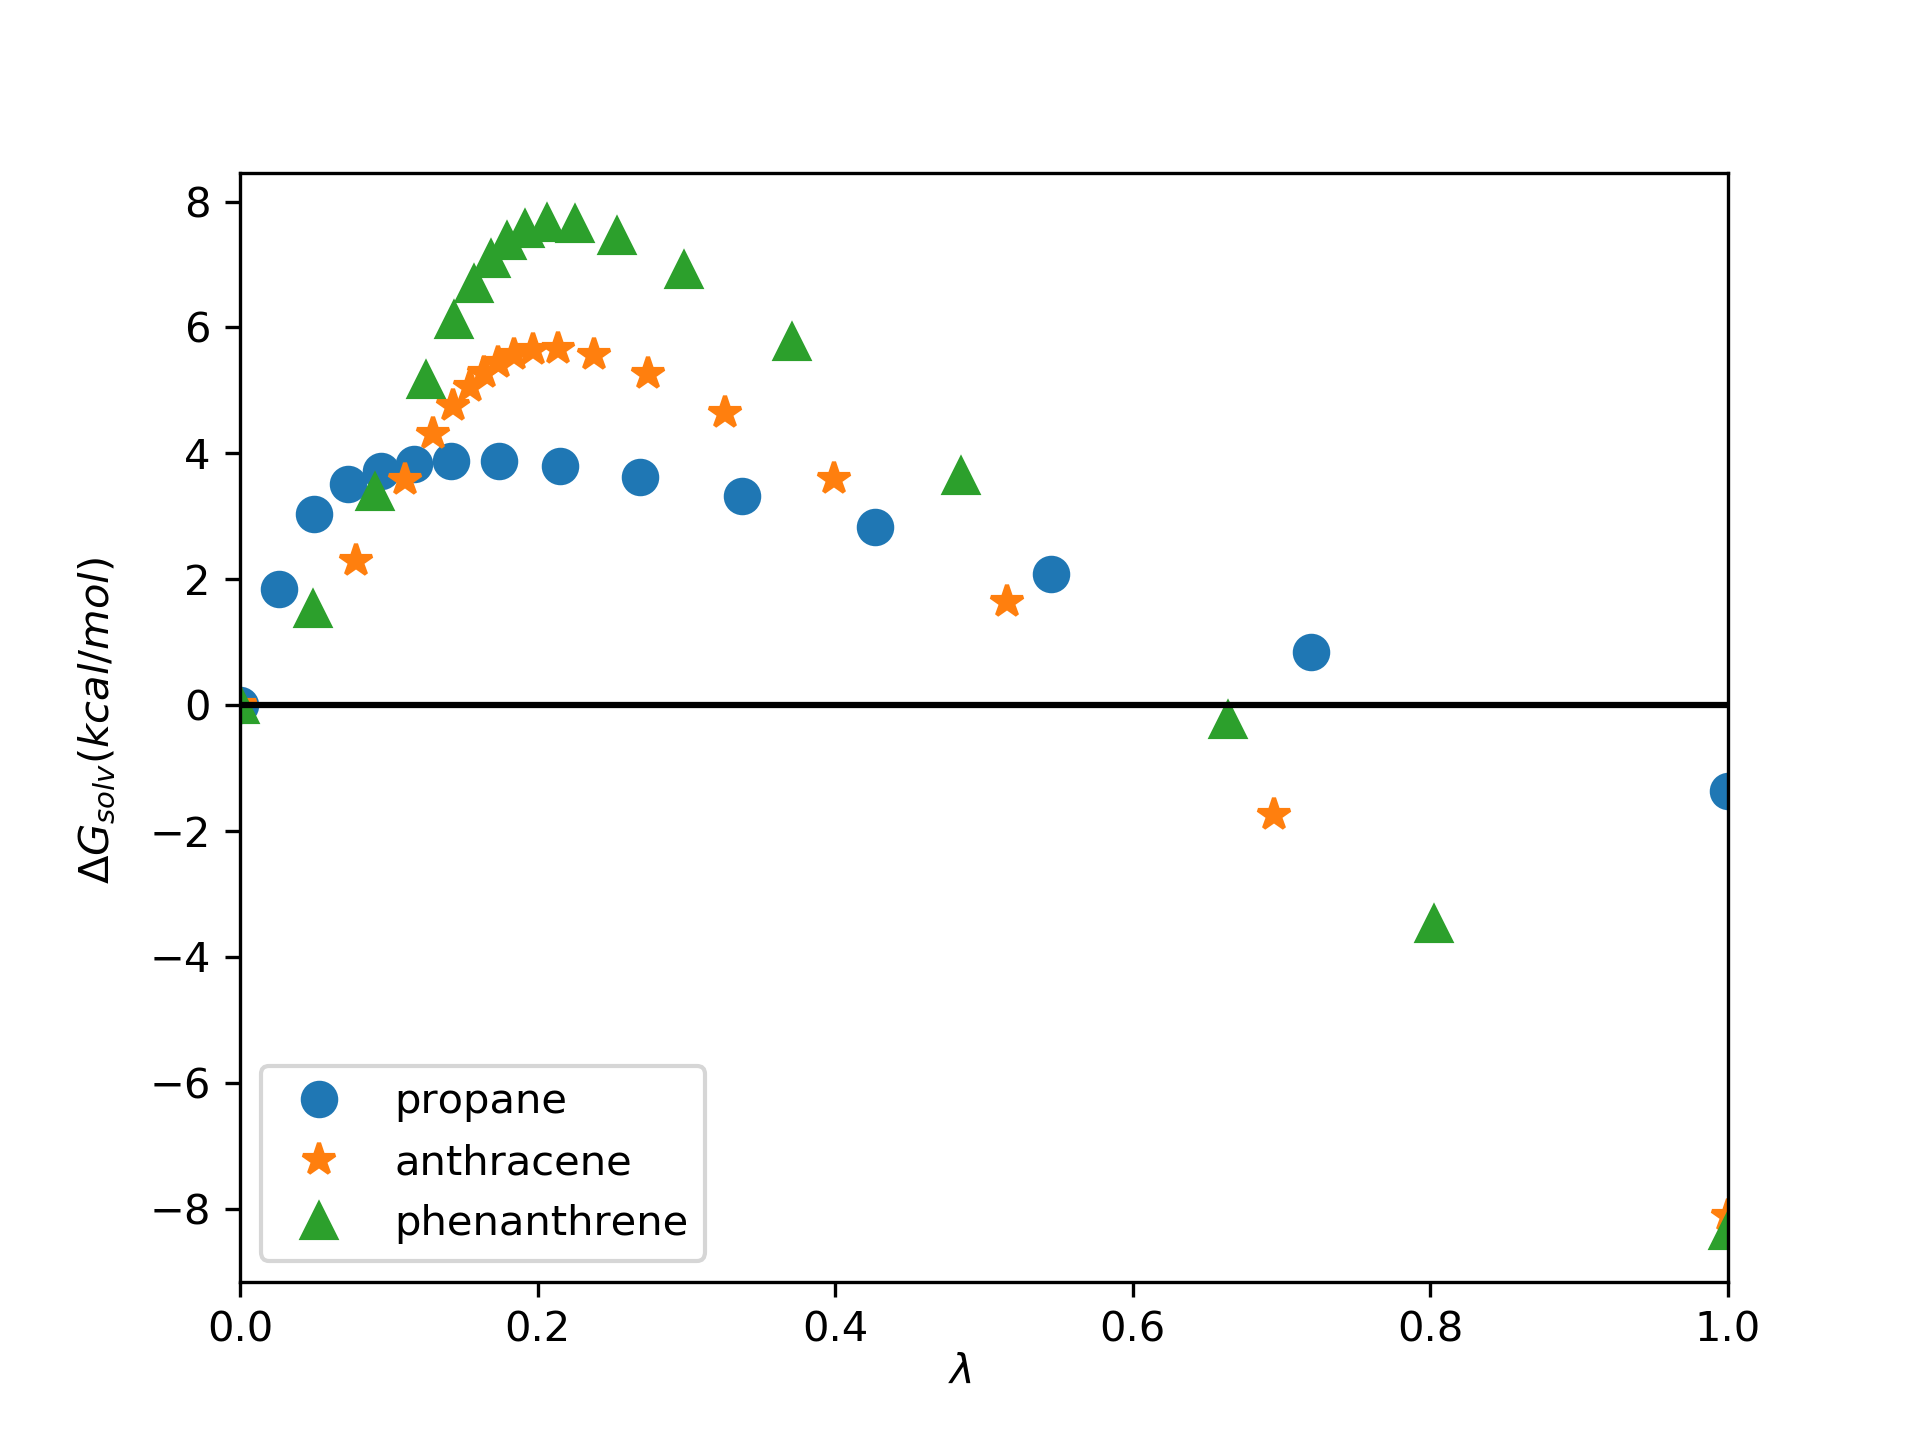
\includegraphics[width=0.9\linewidth]{Figures/oct}
	\caption{Solvation free energy profiles of different solutes in 1-octanol.}
	\label{fig:oct}
\end{figure}

\begin{figure}[H]
	\centering
    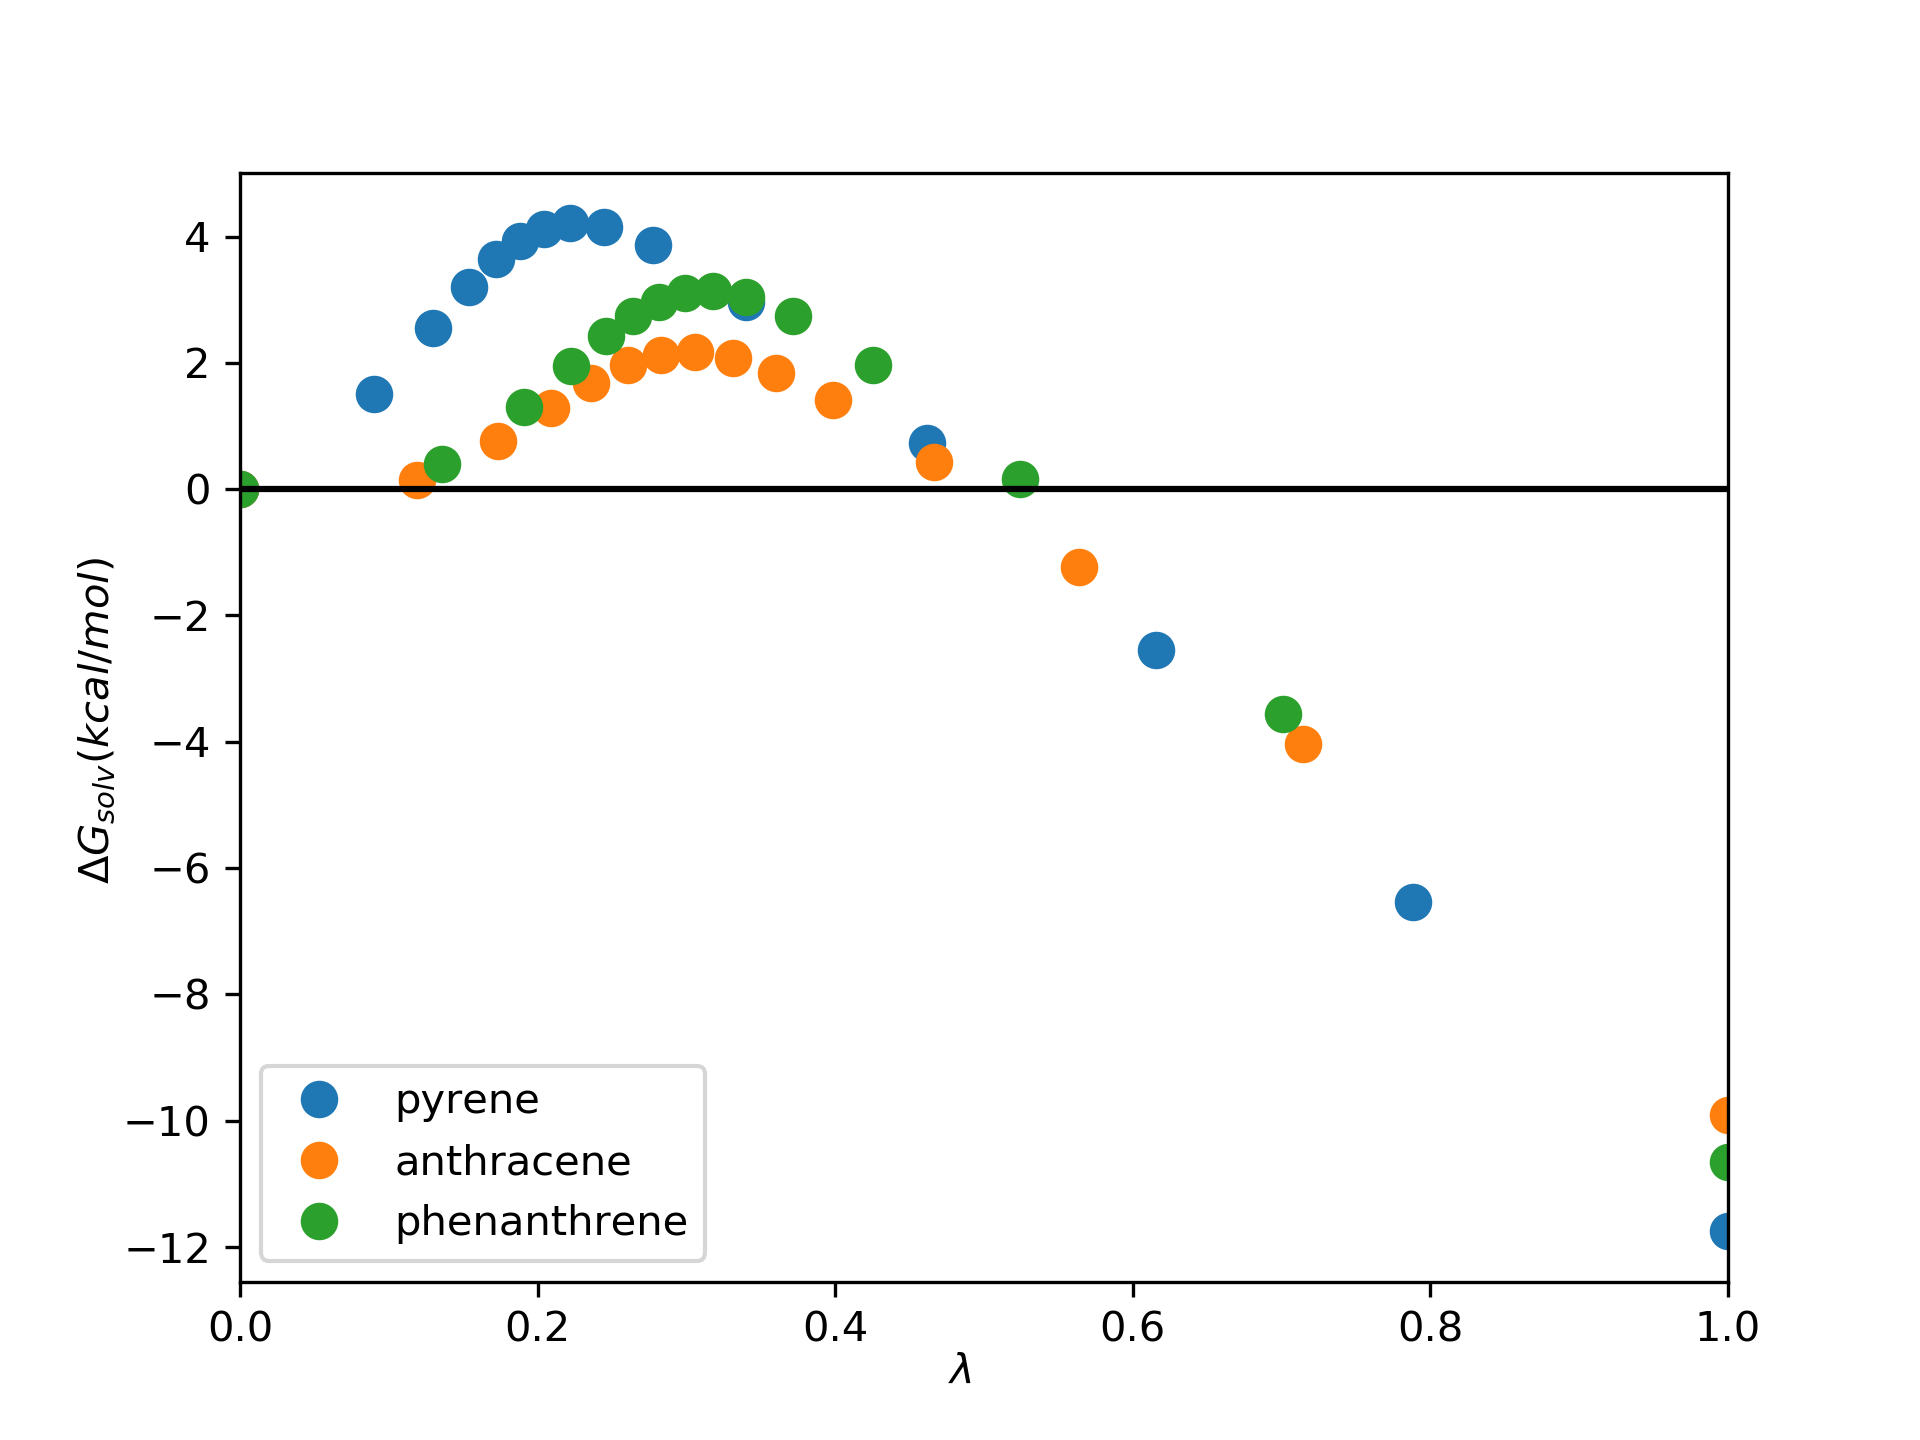
\includegraphics[width=0.9\linewidth]{Figures/tol}
    \caption{Solvation free energy profiles of different solutes in toluene. }
    \label{fig:tol}
\end{figure}

 The results also indicated the prediction capability of the force field for pairs of aromatic solute and solvent. The influence of the molecule's geometry on free energy curves (Figure \ref{fig:tol}) was also observed for these pairs. $\Delta G_{solv}$ was calculated too for phenanthrene in toluene and in toluene+$CO_{2}$. To the best of our knowledge, there was no available experimental data for these solvation free energies, but the previous results for phenanthrene in other solvents and for the pair anthracene+toluene showed that the force field is adequate to describe the solvation phenomenon of phenanthrene in an aromatic solvent. The results for these sets are exposed below: 
 
\FloatBarrier
\begin{table}[H]
\centering
  \caption{Calculated values for the solvation free energy differences (kcal/mol) of phenanthrene in toluene+$CO_{2}$.}
  \label{tbl:solv3}
  \begin{tabular}{ll}
    \hline
      $w_{CO_{2}}$ & $\Delta G_{solv}^{Mie}$ \\
    \hline
    0.0    & -10.65 $\pm$ 0.02   \\
    0.087  & -10.73 $\pm$ 0.02   \\
    0.119  & -10.78 $\pm$ 0.02   \\
    0.169  & -10.71 $\pm$ 0.02   \\
    0.289  & -10.69 $\pm$ 0.02   \\
    \hline
  \end{tabular}
\end{table}
\FloatBarrier

The increasing of $CO_{2}$ mass fraction in toluene caused a small effect on solvation free energies. First, the $\Delta G_{solv}$ decreased with the increase of $w_{CO_{2}}$ , indicating a higher solubility. From the 0.169 fraction, the effect was reversed and carbon dioxide became an anti solvent. It was observed that asphaltene precipitation occurs when carbon dioxide mass fractions became higher than 0.10 in the system asphaltene+toluene+carbon dioxide \cite{SOROUSH2014405}, what is in accordance with the anti solvent effect of carbon dioxide observed on the calculated values. It is also important to point out that the small differences observed in the free energy profiles (Figure \ref{fig:Figure_1}) may indicate the non-influence of $CO_{2}$ in solvation of phenanthrene in toluene when using the Saft-$\gamma$ Mie force field. But, since this is a qualitative study due the lack of this system experimental data, more studies need to be done in order to make a secure assertion about it.   

\begin{figure}[H]
\centering
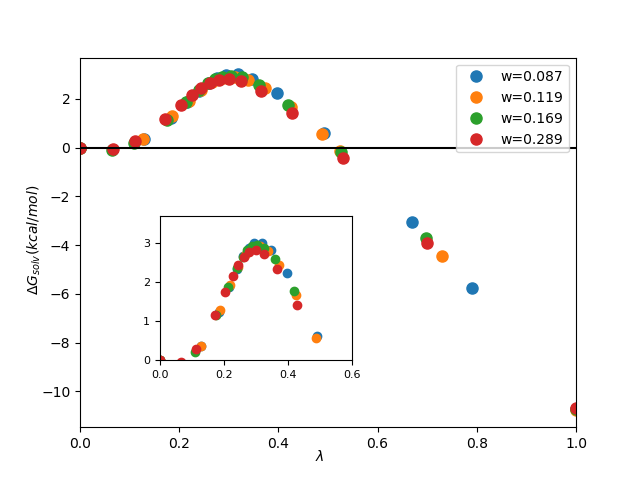
\includegraphics[width=0.9\linewidth]{Figures/Figure_1}
\caption{Solvation free energy profiles of phenanthrene in toluene+$CO_{2}$.}
\label{fig:Figure_1}
\end{figure}


\section{Hydration free energies}

The hydration free energies of widely studied solutes (propane, benzene) and aromatic solutes (toluene, phenanthrene) were calculated with a group of fifteen intermediate states. First, the binary interaction parameter was set to zero, but the results obtained deviated a lot from the experimental data as can be seen in the table below:

\FloatBarrier
\begin{table*}[h]
	\centering
	\caption{Calculated values for the hydration free energy differences (kcal/mol) of solutes in water for $k_{ij}=0$.}
	\label{tbl:solv3}
	\begin{tabular}{lll}
		\hline
		Solute & $\Delta G_{solv}^{Mie}$ & $\Delta G_{solv}^{exp}$ \\
		\hline
		propane   & 2.00 $\pm$ 0.20&1.10 $\pm$ 0.01   \\
		benzene  & -0.86 $\pm$ 0.20 & -4.45 $\pm$ 0.03   \\
		toluene  & -0.83 $\pm$ 0.20 &-15.80 $\pm$ 0.06   \\
		phenanthrene & -3.88 $\pm$ 0.60 &-10.90 $\pm$ 0.04   \\
		\hline
	\end{tabular}
\end{table*}
\FloatBarrier

After these results, the need of  the binary interaction parameter was clear. The $k_{ij}$ estimation with the SAFT VR Mie EoS and experimental vapor pressure data also didn't provide good results, then the strategy of estimating the $k_{ij}$ with the output from solvation free energy calculations with molecular dynamics was used, as described in the last paragraph of section \ref{solvme}.  Individual values for the interaction parameter for each solvent was initially found, but, since the parameters values for aromatic solutes were very similar (0.148, 0.162, 0.152), the average of these values was taken in order to obtain a general parameter for the water+aromatic pairs. The parameters estimated are:

\begin{table*}[h]
  \centering
  \caption{Binary interaction parameters employed.}
  \label{tbl:kij}
  \begin{tabular}{ll}
    \hline
      Pair & $k_{ij}$ \\
    \hline
    water  + propane      & 0.067  \\
    water  + aromatic      & 0.154 \\  
    \hline
  \end{tabular}
\end{table*}

The relatively large $k_{ij}$ value for the aromatic solutes can be pinned on the lack of an explicit association term on the model and on the water model itself, since the model didn't need a $k_{ij}$ for mixtures with 1-octanol. Nevertheless, the value obtained by fitting the parameter with molecular dynamics interfacial tension data was larger for the mixture water+toluene (0.241) \cite{herdes2017}.  The SAFT-$\gamma$ Mie model for water \cite{lobanova2016} has actually two different of temperature dependent sets of parameters. The one used in this work was the set estimated with experimental interfacial tension data, but the binary interaction parameter estimated with MD phenomenon tension data could not be transferable to solvation free energy calculations. Modeling the water with a coarse grained methodology has a lot of difficulties because the water molecules move independently and only have non bonded interactions \cite{hadley2010,hadley2012}. The  SAFT-$\gamma$ Mie water model considers that one water molecule corresponds to one bead, this strategy only saves small simulation time, but it is able to predict properties at physiological temperatures unlike other more aggressive models, which consider that one bead represents various water molecules. In light of all this, the SAFT-$\gamma$ Mie force field appears to be a good alternative when working close to room temperatures, but the necessity of additional parameters estimated with molecular simulation indicates problems on the model. The solvation free energy differences calculated with the final fitted binary interaction parameters are presented in Table \ref{tbl:solv2}.  

\begin{table}[H]
  \centering
  \caption{Calculated and experimental values for the hydration free energy differences  (kcal/mol) of solutes in water.}
  \label{tbl:solv2}
  \begin{tabular}{lllll}
    \hline
     Solute      & $\Delta G_{solv}^{exp}$ & $\Delta G_{solv}^{Mie}$ & Absolute Deviation & $\Delta G_{solv}^{GAFF}$ \\
    \hline
    propane      &  2.00 $\pm$ 0.20 & 2.01 $\pm$ 0.01& 0.01 &2.50 $\pm$0.02 \\
    benzene      & -0.86 $\pm$ 0.20 & -1.12 $\pm$ 0.01    &  0.26    &-0.81$\pm$0.02 \\  
    toluene      & -0.83 $\pm$ 0.20 & -0.84 $\pm$ 0.01   &  0.01    &-0.79$\pm$0.03\\
    phenanthrene & -3.88 $\pm$ 0.60 & -3.47 $\pm$ 0.02& 0.41 &-5.26$\pm$0.03 \\
    \hline
%    RMSE         &                  &               &  0.24     &      \\
%    \hline
  \end{tabular}

\end{table}

Hydration free energy differences with $k_{ij}$ had low absolute deviations from the experimental data, as expected since the parameter was adjusted to fit the data. The root mean square error (RMSE) for the pairs tested with the SAFT-$\gamma$ 	Mie model was equal to 0.24, meanwhile the RMSE for hydration free energy differences with the GAFF force field \cite{PMID:24928188} was 0.73. The difference in absolute deviations between the two force fields is significantly high for phenanthrene, hence the coarse grained force field with a binary parameter is preferred if the application requires a higher level of accuracy. Hydration free energy profiles in Figure \ref{fig:water} show the geometry  dependence on the free energy profiles. We can observe also that the solvation free energy for the first non zero lambda is negative for benzene and toluene, when a positive value is expected.This can be caused by numerical errors or by the force field. 


\begin{figure}[H]
\centering
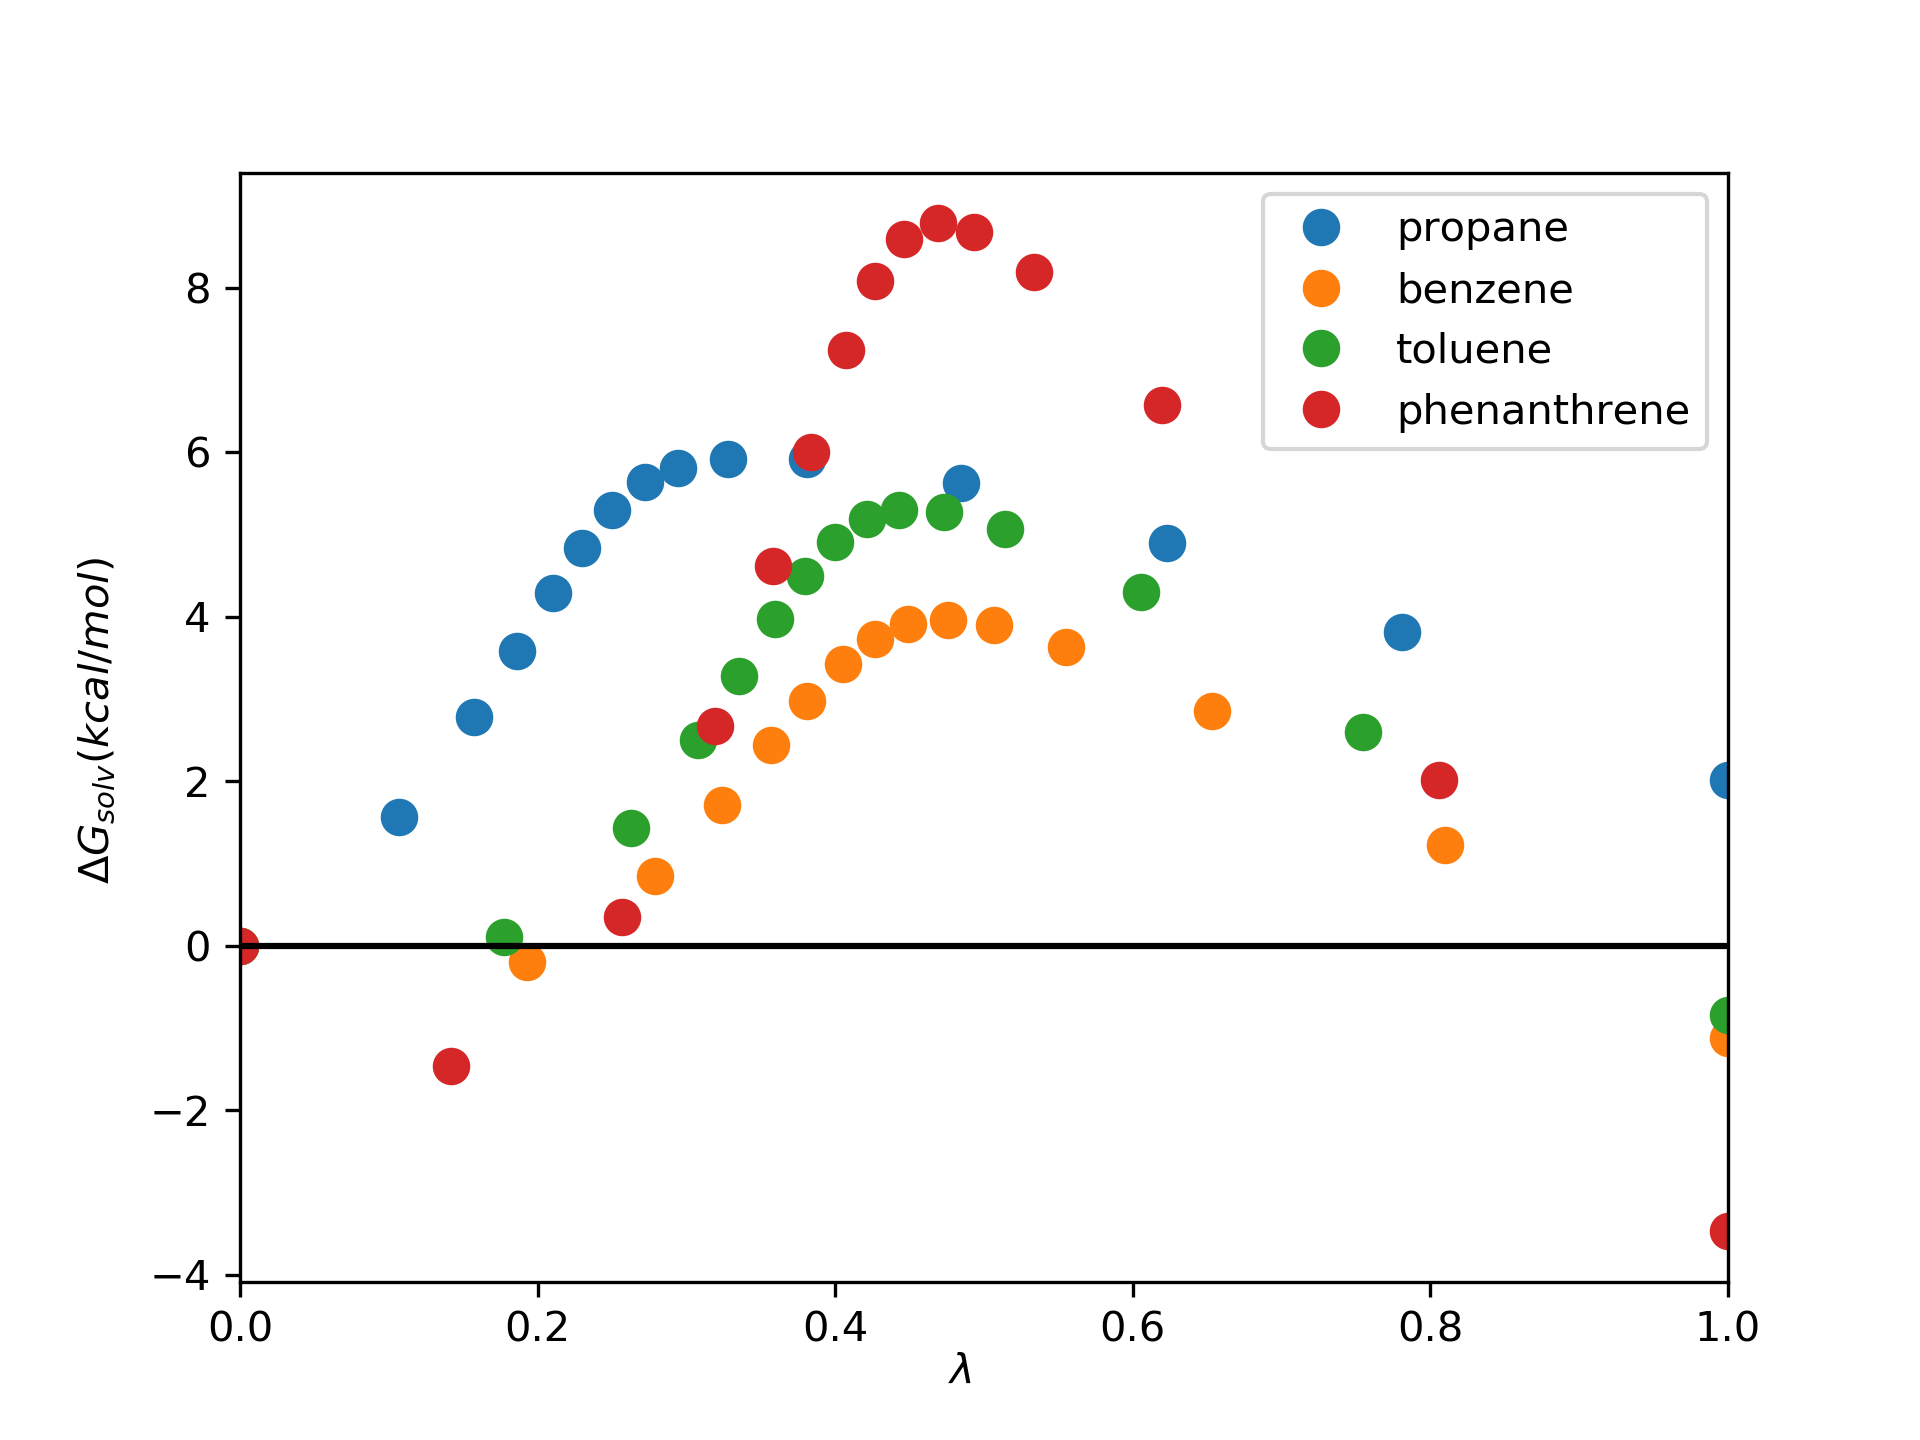
\includegraphics[width=0.9\textwidth]{Figures/water}
\caption{Hydration free energy profiles for different solutes.}
\label{fig:water}
\end{figure}


